%*****************************************************************
%*************************** Section 8 ***************************
%************************ Verteilerplatine ***********************
%*****************************************************************


\pagestyle{fancy}
\rhead{\thepage} \chead{} \lhead{\ref{Sec8}. \nameref{Sec8}}
\cfoot{}

\section{Verteilerplatinen}\label{Sec8}

Anders als beim Fahrzeug von Herrn Arne Kullina werden bei dieser Fahrzeugversion zwei statt nur einer Verteilerplatine verbaut. Die Leistungsverteilung findet auf der Grundplatte platz und die steckbare Verteilung der Signale für die Fahrzeugperipherie auf der oberen Ebene. 

\subsection{Leistungsverteiler auf der unteren Fahrzeugebene}\label{Sec8Sub1}

\begin{minipage}[t]{0.47\textwidth}
Von der Leistungsverteilerplatine auf der unteren Fahrzeugebene (siehe Abbildung \ref{fig:Leistungsverteilerplatine}) wird die gesamte Fahrzeugperipherie mit der Batteriespannung versorgt. Sowohl der Schaltspannungsregler für die Spannungsversorgung der Servo-Lenkung, als auch der Linearspannungsregler auf der oberen Verteilerplatine und die \acp{ESC} erhalten hier ihre Versorgungsspannung. Der Vorteil, dass auf der Grundplatte lediglich der Versorgungsspannungsabgriff erfolgt, liegt darin, dass das Fahrzeug seltener zerlegt werden muss. Da auf der Grundplatte keine wichtige Schaltung verbaut ist, können die meisten Probleme gelöst werden, ohne auf die untere Fahrzeugebene zugreifen zu müssen.
\end{minipage}
\begin{minipage}[t]{0.47\textwidth}
\vspace{-7mm}
\begin{figure}[H] %H für Positionierung hier
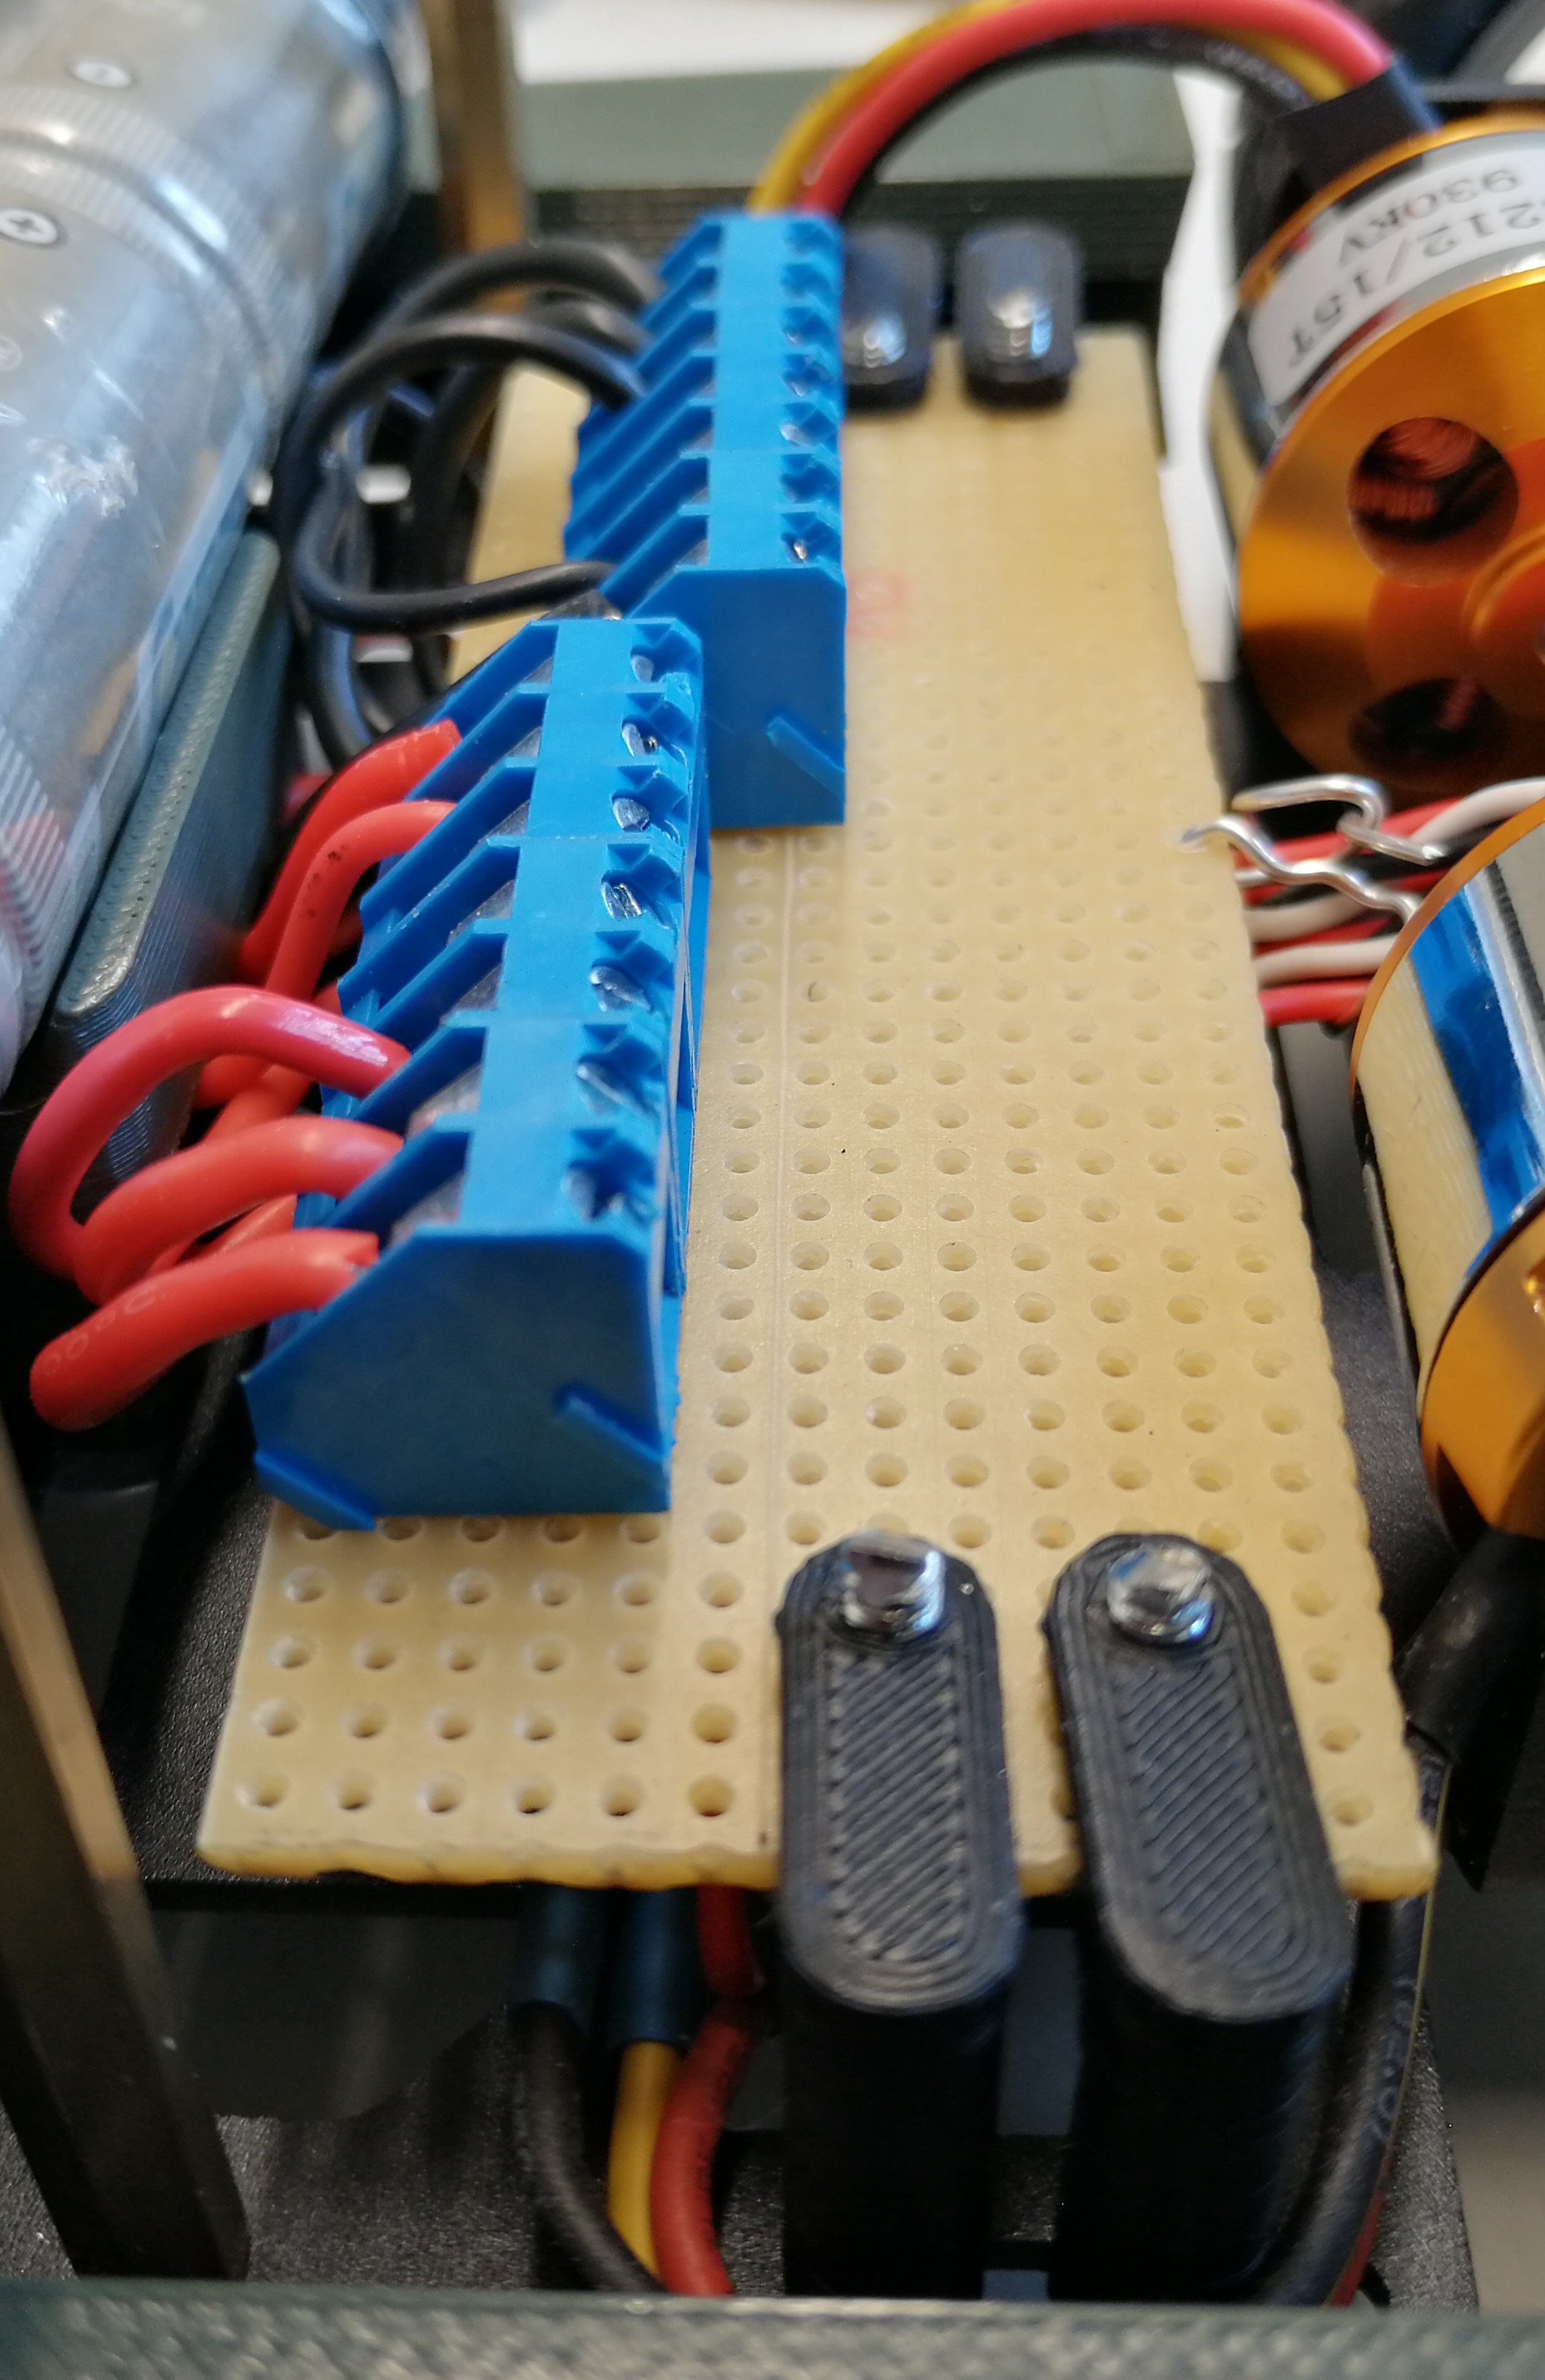
\includegraphics[width=.7\textwidth]{sec8/images/Leistungsverteilerplatine} 
\centering
\captionsetup{width=.9\textwidth}
\caption[Leistungsverteilerplatine auf der unteren Fahrzeugebene]{Leistungsverteilerplatine auf der unteren Fahrzeugebene}
\centering
\label{fig:Leistungsverteilerplatine}
\end{figure}
\end{minipage}


\subsection{Signalverteilerplatine auf der oberen Fahrzeugebene}\label{Sec8Sub2}

Auf der Signalvertielerplatine befindet sich außer der Drehzahlmessung (siehe Kapitel \ref{Sec4Sub5}) auch die Verteilung der PWM-Signale der Antriebe und Servo-Lenkung und der Linearspannungsregler für die Spannungsversorgung des Controllers. In der Abbildung \ref{fig:Signalverteilerplatine} ist die gesamte Platine zu sehen. Die Drehzahlmessung ist in rosa hervorgehoben, die Versorgung der Servo-Lenkung in grün, die PWM-Signalverteilung des linken und rechten Antriebs in orange und violett, der Linearspannungsregler in braun, dessen Versorgung von der Leistungsverteilerplatine in rot und die Versorgungsspannungsanschlüsse des Controllers in grau. 


\begin{figure}[H] %H für Positionierung hier
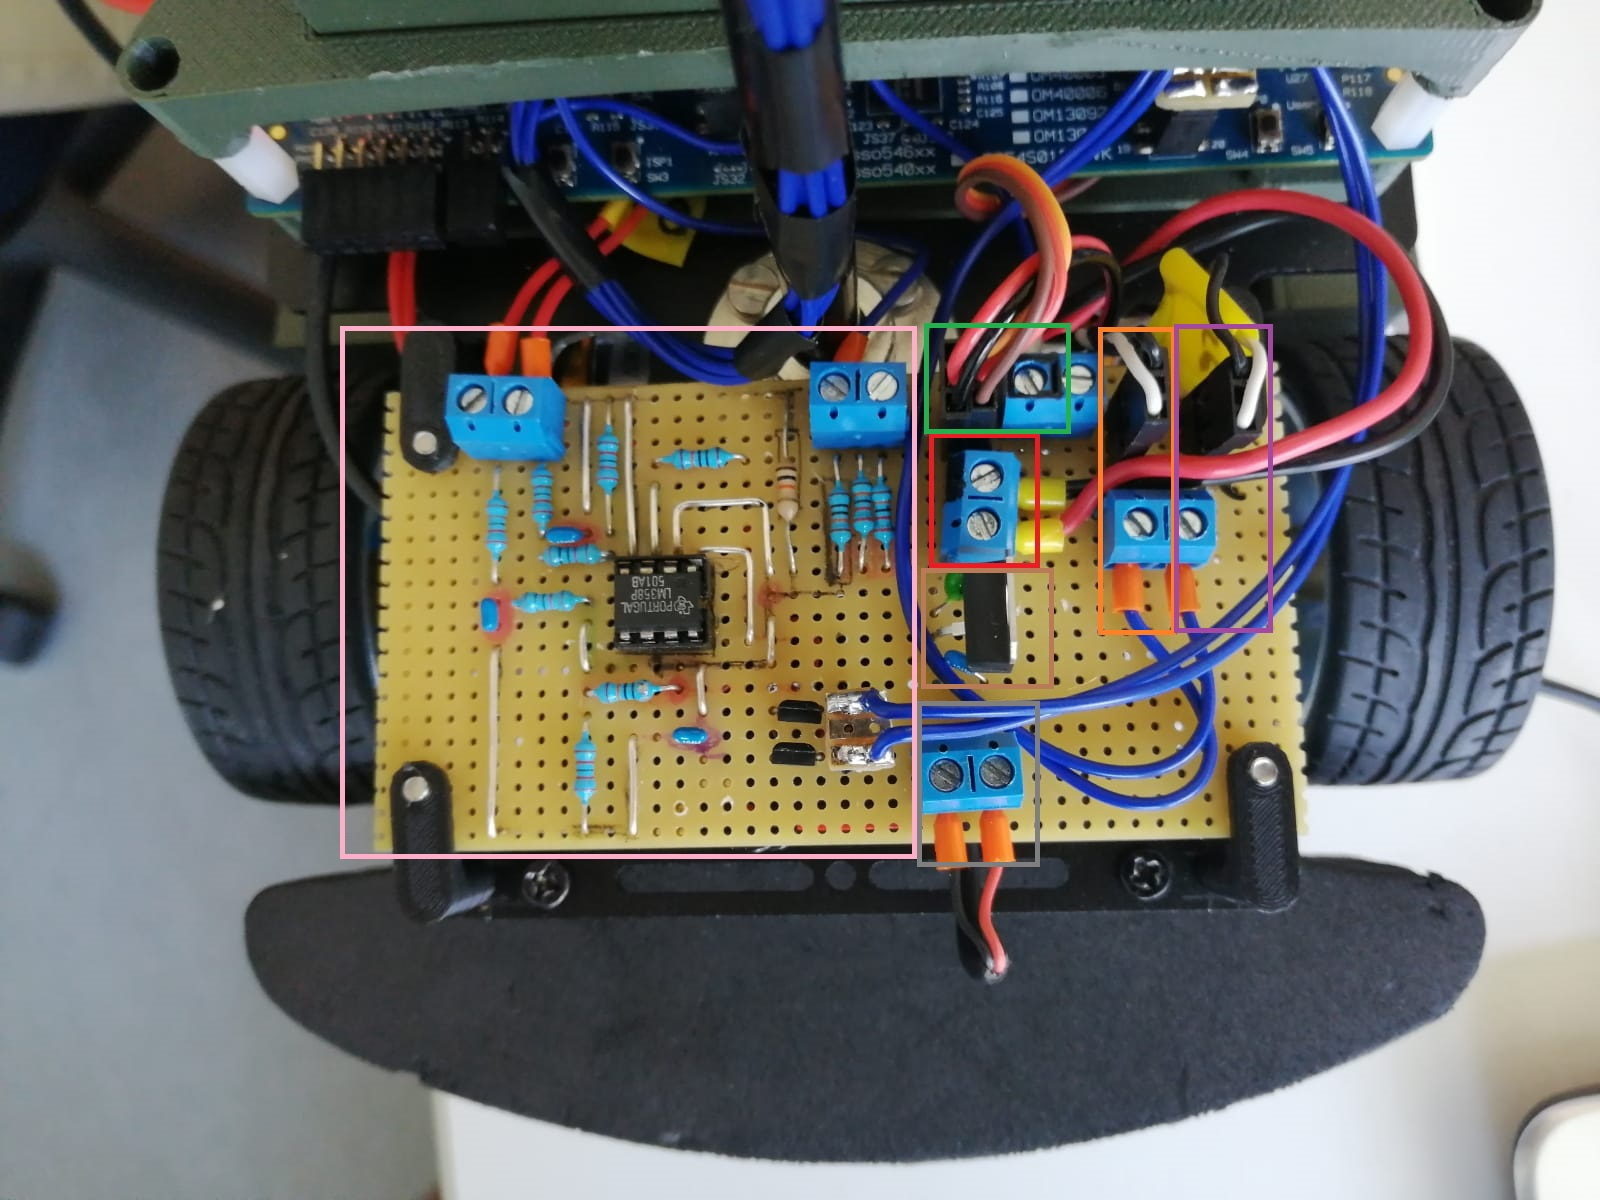
\includegraphics[width=.7\textwidth]{sec8/images/Signalverteilerplatine} 
\centering
\captionsetup{width=.9\textwidth}
\caption[Signalverteilerplatine auf der oberen Fahrzeugebene]{Signalverteilerplatine auf der oberen Fahrzeugebene}
\centering
\label{fig:Signalverteilerplatine}
\end{figure}


\newpage